\section{Cell Movement}

% 5 marks for definitions of distributions and reasons behind the choice of distribution

The random movement of cells can be modelled using a probability distribution.
Probability distributions can be classified as discrete or continuous, we will assess uniform and Bernoulli type distributions.
The uniform distribution is usually regarded as a continuous distribution but can also be used to model discrete variables,
all values are equally likely to be selected.
% hence it is a good choice for the random movement of cells.
The Bernoulli distribution is a discrete distribution that models a single trial with two outcomes,
the probability of the two outcomes is $p$ and $1-p$.
% hence it is not suitable for the random movement of cells.

% The Beta distribution is a continuous distribution that models the probability of a value between 0 and 1.

% Area under the graph is one

% \[ f(x) =\begin{cases}a & \text{if } x = 1\\b & \text{if } x = 0\end{cases}\]

% \[ f(x) =\begin{cases}1 & \text{for } 0  \leq x  \leq  1\\0 & \text{otherwise}\end{cases}\]

% Uniform distribution
% Definition of distributions
% Uniform distributions
% Bernoulli Distribution

% Bias introduced with different distributions

When all directions are equally probable a uniform distribution should be used.
If a Bernoulli distribution was selected, it would introduce a bias to the direction of movement.
This could be desired in a complex model where factors such as surface tension affect the direction taken by the cell.

The algorithm for random walk shall generate a list of available directions (\autoref{lst:moveCell}) and select one at random (\autoref{lst:availableNormal} and \autoref{lst:availableDiagonal}).
Two different methods of movement shall be compared, a square movement and a diagonal movement.

% how random numbers are actually generated in rust

\subsection{Simulation Plots}

Both directions have bias, square moves to the right and diagonal moves downwards.
This is because the number generation is random and hence direction is random.
In \autoref{fig:task1} the plots show the same number of steps (100), but the diagonal plot moves further than the square plot.

\begin{figure}[!ht]
    \centering
    \begin{subfigure}{0.4\textwidth}
    	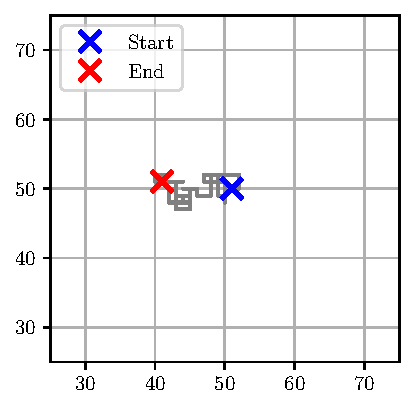
\includegraphics[width=\textwidth]{task1-1}
    	\caption[Square]{Square}
    	\label{fig:task1-1}
    \end{subfigure}
    \begin{subfigure}{0.4\textwidth}
    	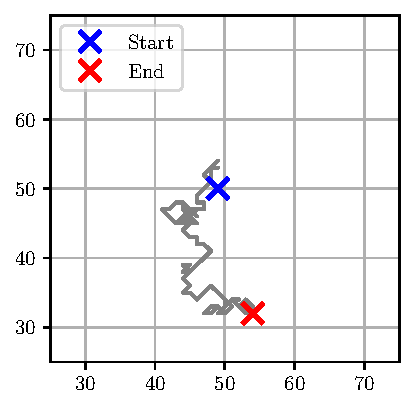
\includegraphics[width=\textwidth]{task1-2}
    	\caption[Diagonal]{Diagonal}
    	\label{fig:task1-2}
	\end{subfigure}
	\caption[Cell movement plots]{Cell movement plots}
    \label{fig:task1}
\end{figure}

\clearpage

\subsection{Simulation Heatmap}

The movement of the cells can be visualized using a heatmap.
Several and end points can be selected using another uniform distribution.
Next the random walk can execute until the end point is reached (\autoref{fig:task1-fill}),
this process can be repeated multiple times to record the visited cells.


The results are shown in \autoref{fig:task1-visited}, there are small hotspots but overall, the distribution is uniform.
With more iterations, the distribution would become more even.
This validates the uniform distribution of both the movements algorithms.
% and validates the uniform distribution of the random start and end points

\begin{figure}[ht]
    \centering
    \begin{subfigure}{0.45\textwidth}
        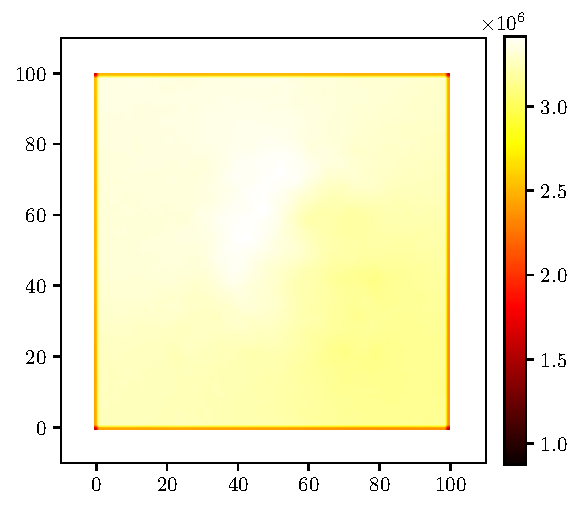
\includegraphics[width=\textwidth]{task1-visited-square}
        \caption[Square]{Square}
        \label{fig:task1-visited-square}
    \end{subfigure}
    \begin{subfigure}{0.45\textwidth}
        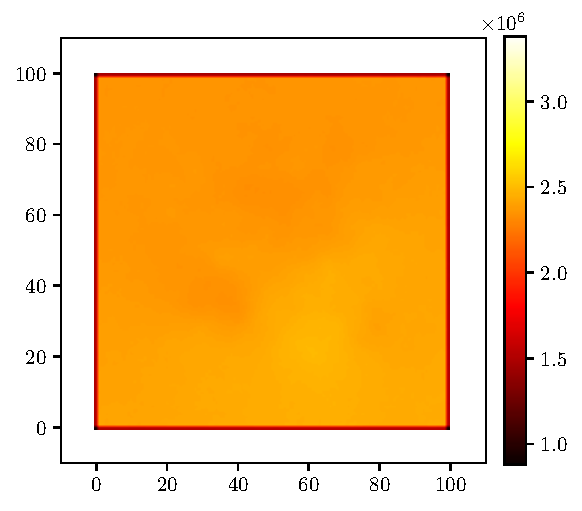
\includegraphics[width=\textwidth]{task1-visited-diagonal}
        \caption[Diagonal]{Diagonal}
        \label{fig:task1-visited-diagonal}
    \end{subfigure}
    \caption[Visited cells simulation heatmap]{Visited cells simulation heatmap}
    \label{fig:task1-visited}
\end{figure}

There is a significant difference in the number of visited cells between the movement types.
This is because the diagonal movement can move further in a single step than the square movement.

The square can perform one step to the left, right, up or down.
The diagonal can perform one step to the left, right, up, down, up-left, up-right, down-left or down-right.
Any diagonal movement is equivalent to $\sqrt{1^2 + 1^2} = \sqrt{2}$ square movements.

Hence square movement is on average $(1 \times 4) / 4 = 1$ steps
The diagonal movement is on average $(\sqrt{2} \times 4 + 1 \times 4) / 8 = 1.2071$ steps
Square is factor of $1 / 1.2071 = 0.8284$ compared to diagonal.

In the sense of moving from one point to another, the diagonal movement is more efficient than the square movement.
This is different from computational complexity.
% However, this is different from computational complexity, where the square movement is more efficient than the diagonal movement.

% TODO - explain the computational complexity of the different movements

% \begin{figure}[ht]
%     \centering
%     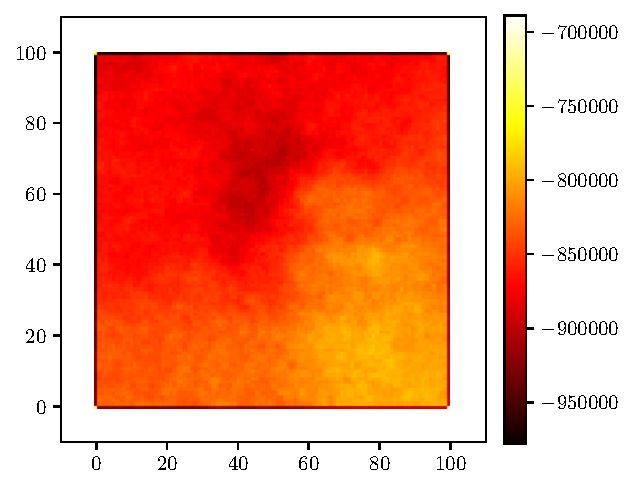
\includegraphics[width=0.45\textwidth]{task1-visited-diff}
%     \caption[Difference in visited cells between square and diagonal simulation heatmap]{Difference in visited cells between square and diagonal simulation heatmap}
%     \label{fig:task1-visited-diff}
% \end{figure}

\clearpage

\begin{figure}[ht]
    \centering
    \begin{subfigure}{\textwidth}
        \centering
        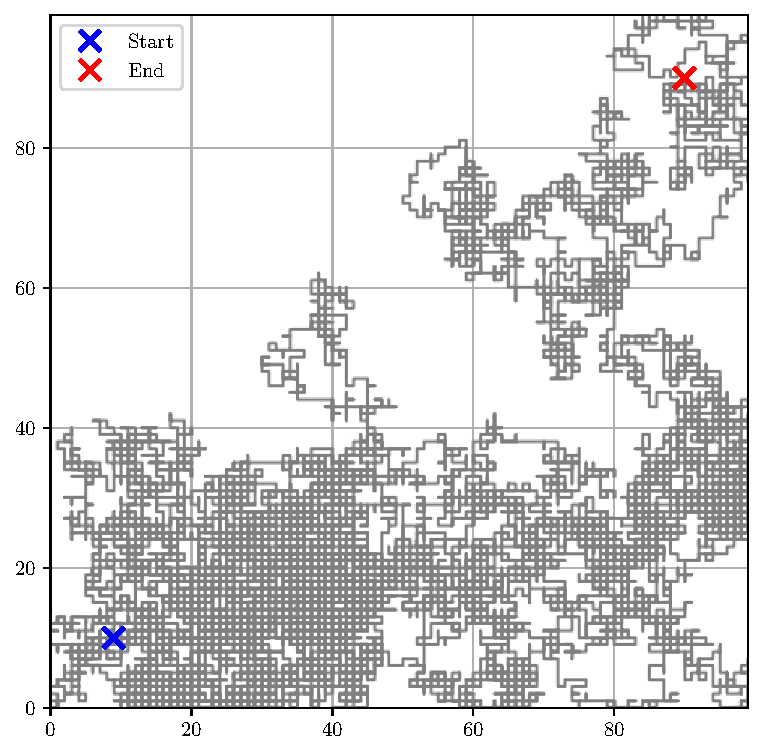
\includegraphics[width=10cm]{task1-1-fill}
        \caption[Square]{Square}
        \label{fig:task1-1-fill}
    \end{subfigure}
    \begin{subfigure}{\textwidth}
        \centering
        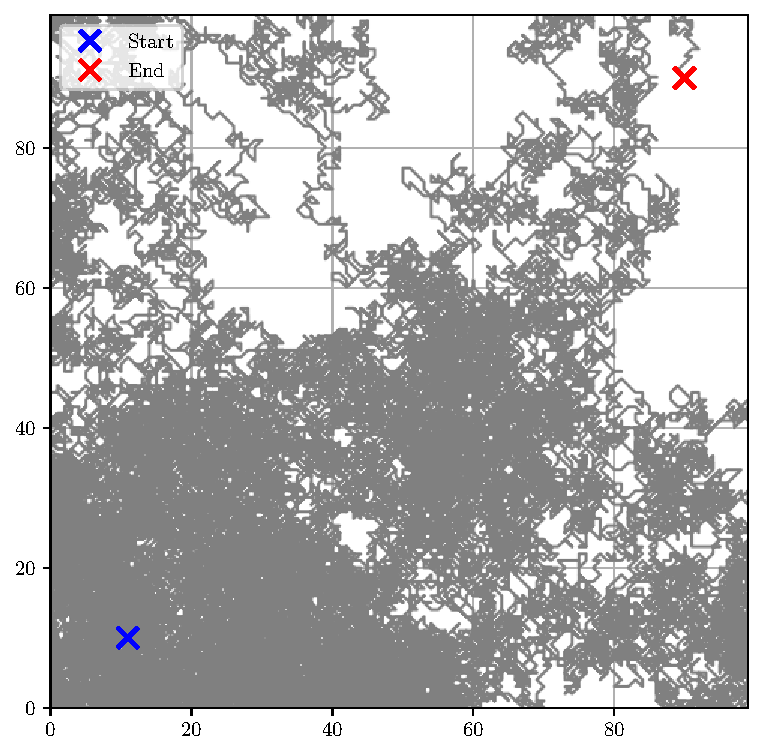
\includegraphics[width=10cm]{task1-2-fill}
        \caption[Diagonal]{Diagonal}
        \label{fig:task1-2-fill}
    \end{subfigure}
    \caption[Cell movement fill plots]{Cell movement fill plots}
    \label{fig:task1-fill}
\end{figure}

\clearpage

\subsection{Movement Complexity}

Using criterion, the computational complexity of the different movements can be measured.
The results are shown in \autoref{fig:move-cell-criterion}.
Square movements take $16.2ns$ compared to diagonal movements which take $42.7ns$, this is a ratio of 0.3794.

\begin{figure}[ht]
    \centering
    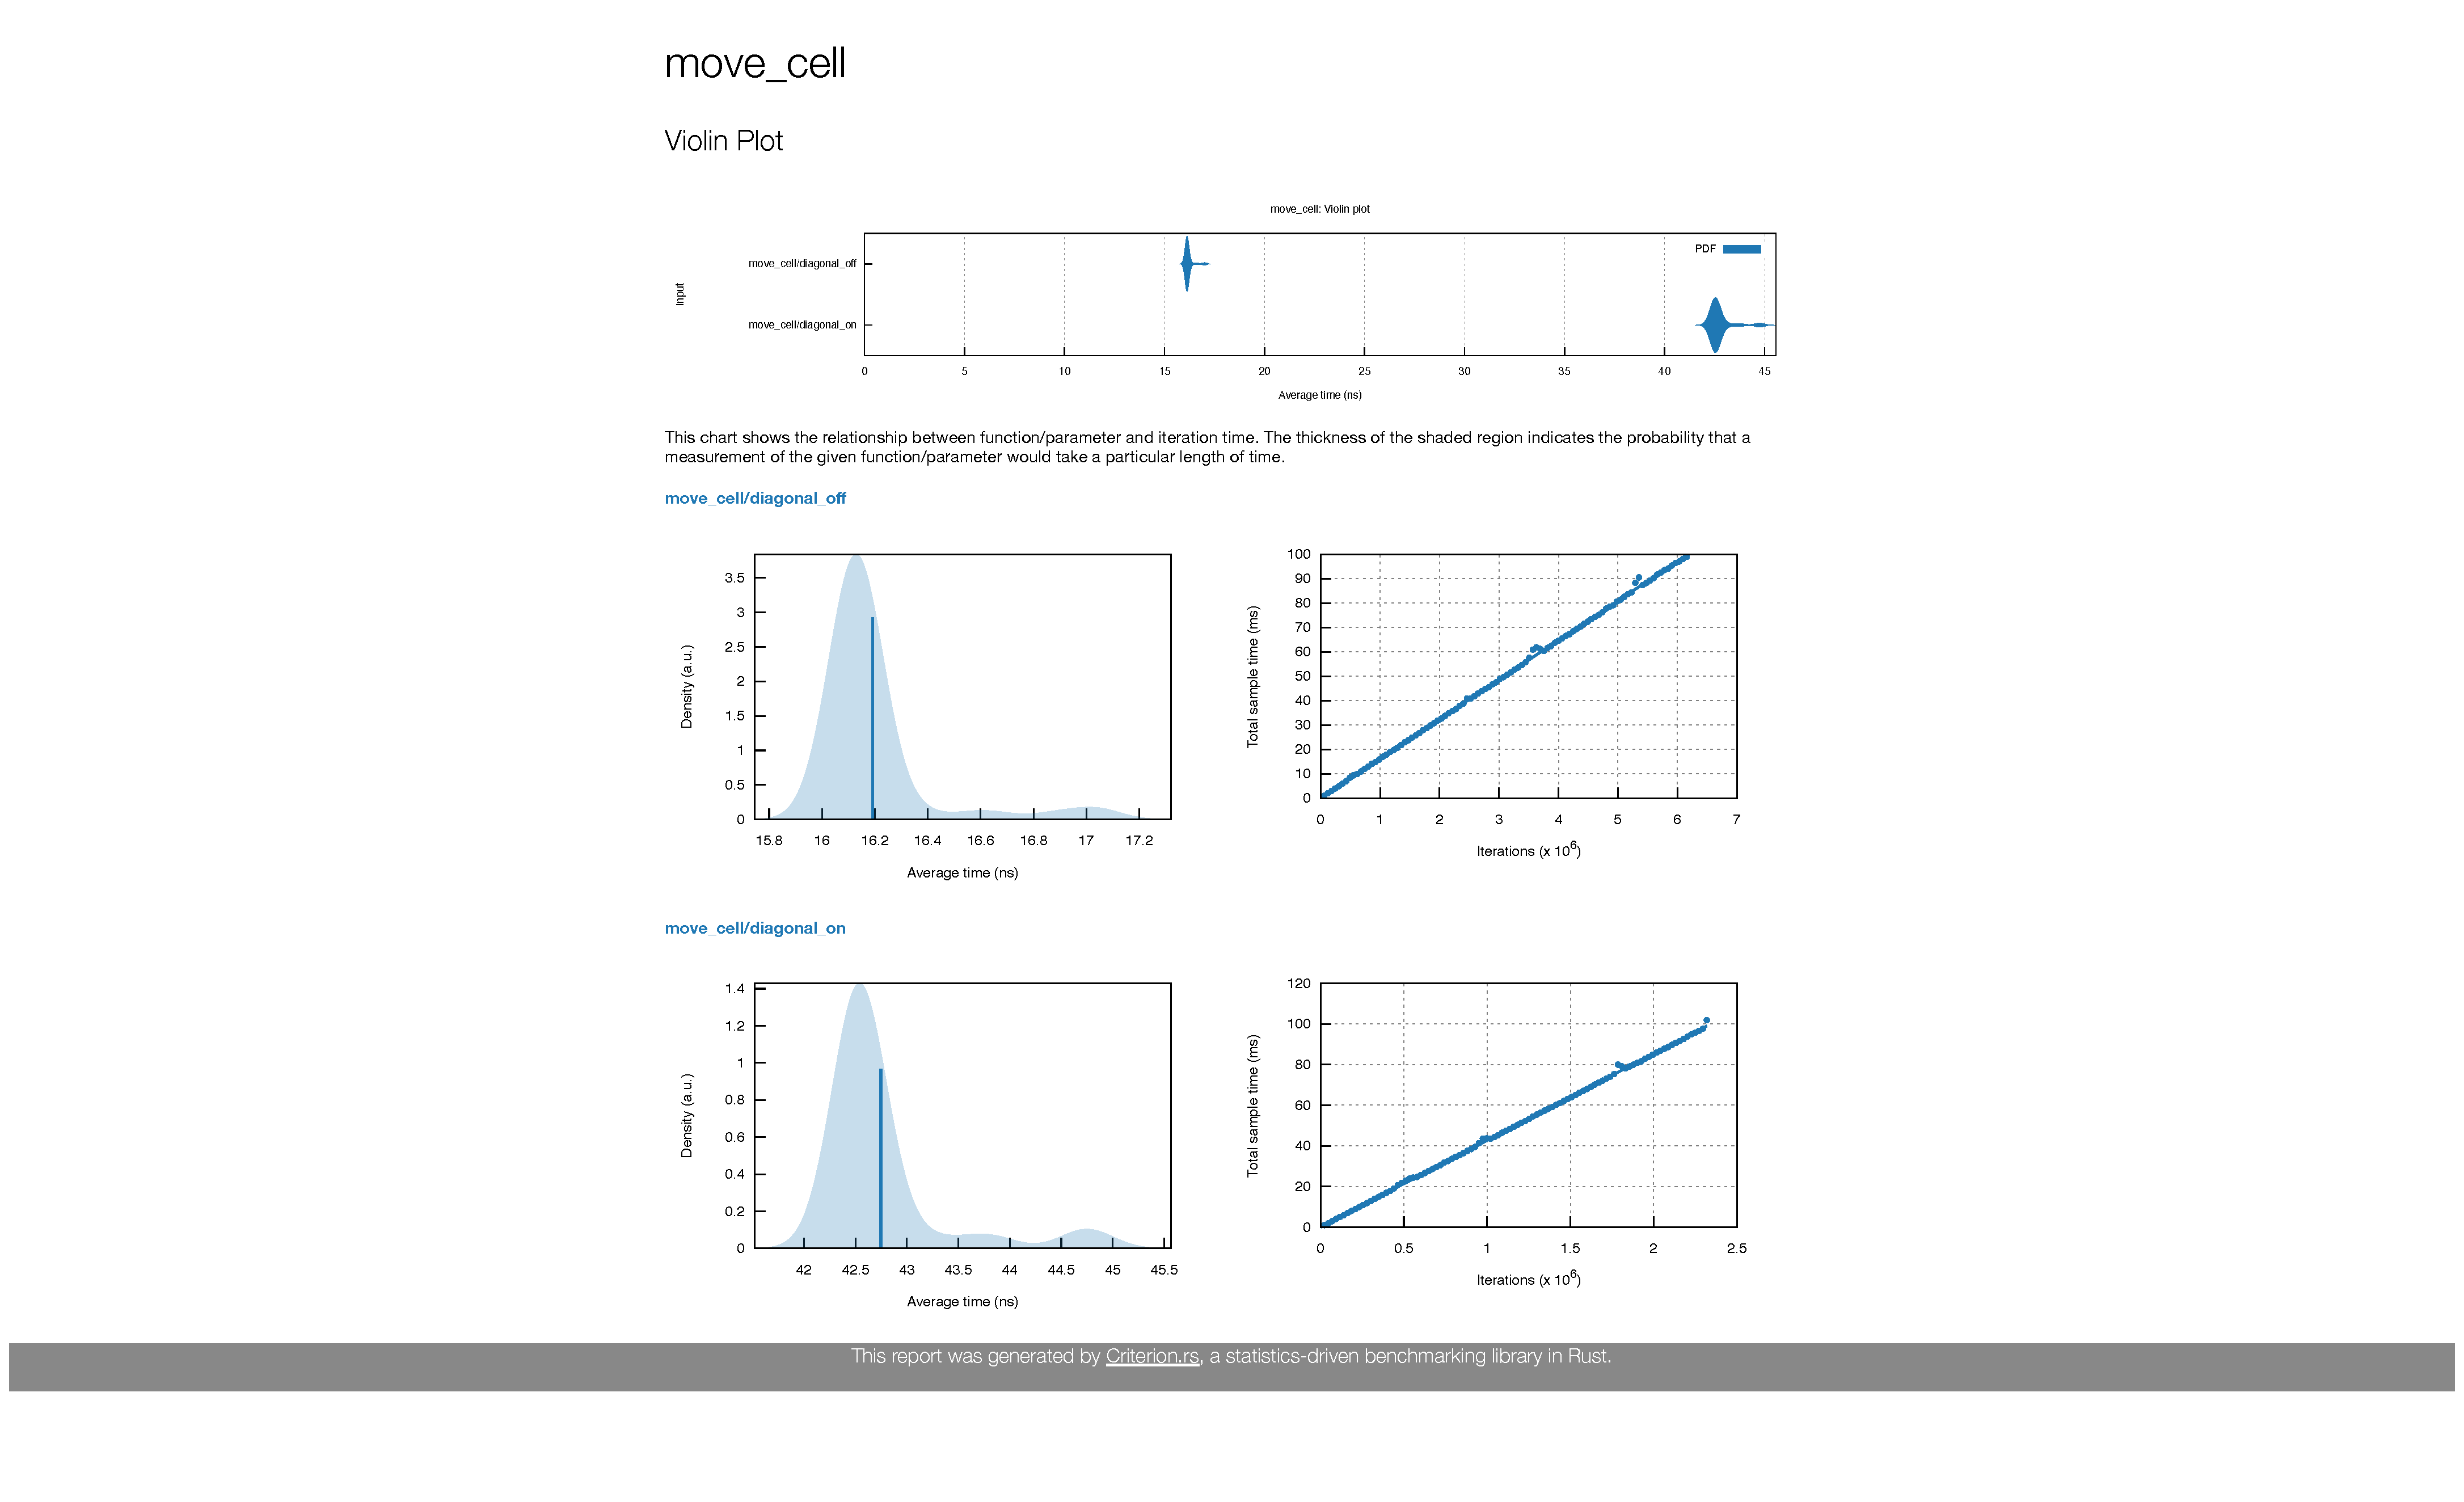
\includegraphics[width=\textwidth, clip, trim=4cm 12cm 1cm 11cm]{move-cell-criterion}
    \caption[Cell movement criterion]{Cell movement criterion}
    \label{fig:move-cell-criterion}
\end{figure}

The diagonal movement is more computationally complex than square movement.
This is because the diagonal movement requires more checks to ensure the cell does not move off the grid.
The act of generating a random number is the same for both movements as a single number is generated to determine the direction of travel.

As single move is of complexity $O(1)$, the complexity of multiple moves is $O(n)$ where $n$ is the number of steps taken.

\clearpage

\subsection{Simulation Steps}

By selecting a random start and end point, we can compare the number of steps and time taken by the square and diagonal movements directly.
If this movement simulation is performed multiple times, the average number of steps and time taken by the two movements can be compared.

Given enough iterations, the average should stabilize and the difference in the number of steps and time taken by the movements can be calculated.

\begin{figure}[ht]
    \centering
    \begin{subfigure}{\textwidth}
        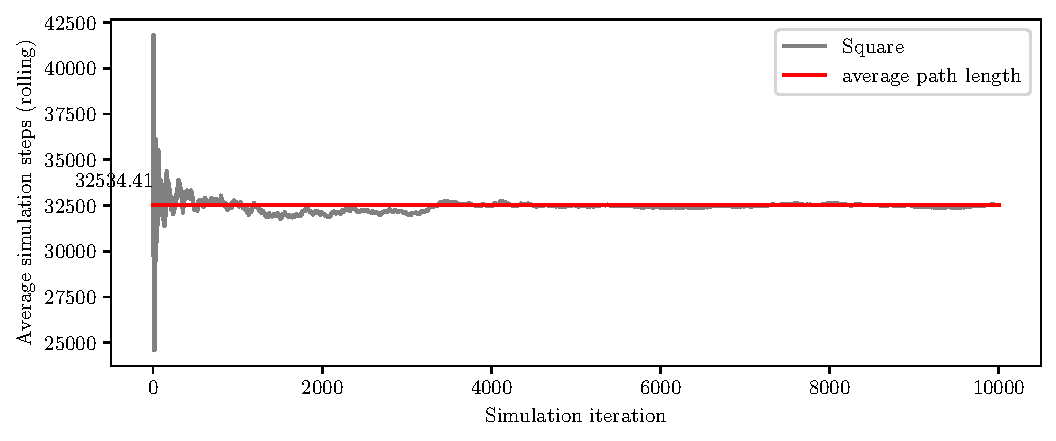
\includegraphics[width=\textwidth]{task1-compare-square-roll}
        \caption[Square]{Square}
        \label{fig:task1-compare-square-roll}
    \end{subfigure}

    \begin{subfigure}{\textwidth}
        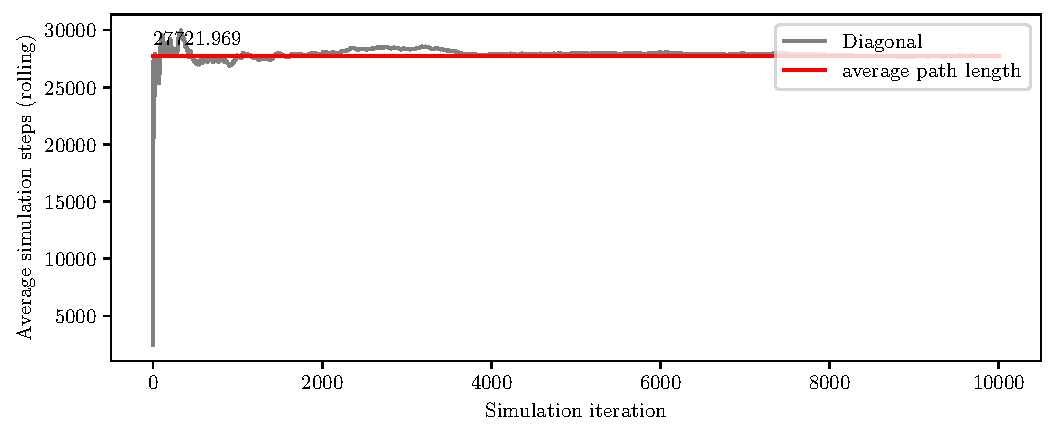
\includegraphics[width=\textwidth]{task1-compare-diagonal-roll}
        \caption[Diagonal]{Diagonal}
        \label{fig:task1-compare-diagonal-roll}
    \end{subfigure}

    \caption[Comparison of square and diagonal simulation steps]{Comparison of square and diagonal simulation steps}
    \label{fig:task1-compare-roll}
\end{figure}

\autoref{fig:task1-compare-roll} shows the number of steps taken by the movements for a single simulation with start and end points of (42, 28) and (29, 74).

% Diagonal - (42, 28) - (29, 74)

As suggested in the previous sections, the diagonal movement takes less steps than the square movement to reach the end point.
However, the diagonal movement takes longer (time) as the computational complexity is higher.

% Plotting on to the same graph...

% \begin{figure}[ht]
%     \centering
%     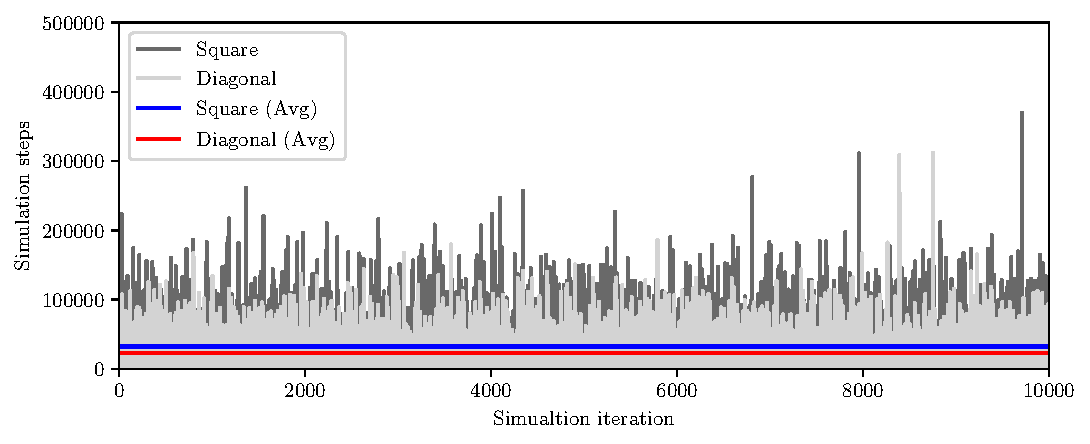
\includegraphics[width=14cm]{task1-compare-single}
%     \caption[Comparison of square and diagonal simulation steps]{Comparison of square and diagonal simulation steps}
%     \label{fig:task1-compare-single}
% \end{figure}

\clearpage

By taking the same process and applying it to a random selection of points, 
the average number of steps and time taken by the movements can be compared for different distances travelled (\autoref{fig:task1-compare}).

% By also measuring the time taken for the simulation to complete allows the computational complexity of the different movements to be compared.
% By plotting the average number of steps against the distance between the start and end points...
% we can establish an average difference in the number of steps taken by the square and diagonal movements.


\begin{figure}[ht]
    \centering
    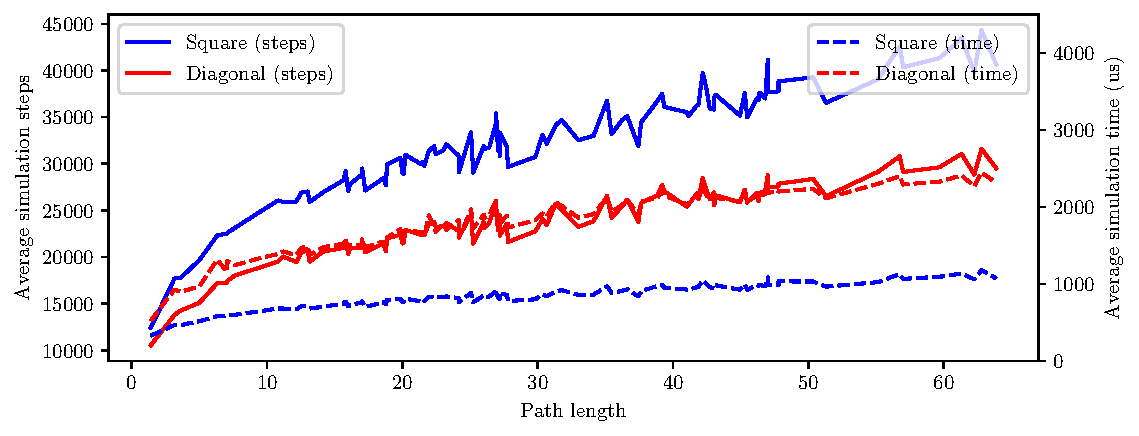
\includegraphics[width=14cm]{task1-compare}
    \caption[Comparison of multiple square and diagonal simulation steps]{Comparison of multiple square and diagonal simulation steps}
    \label{fig:task1-compare}
\end{figure}

Next, by plotting the ratio of the average number of steps and time taken by movements
we can establish a factor by which the diagonal movement is more efficient than the square movement (\autoref{fig:task1-factor-length}).

\begin{figure}[ht]
    \centering
    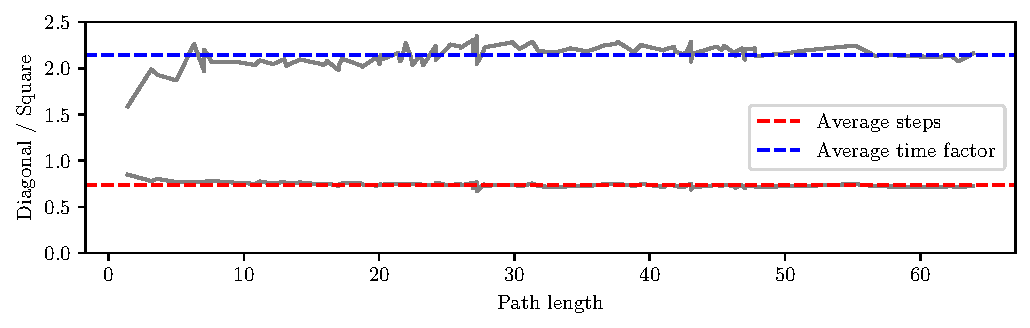
\includegraphics[width=14cm]{task1-factor-length}
    \caption[Comparison of multiple square and diagonal simulation steps (factor length)]{Comparison of multiple square and diagonal simulation steps (factor length)}
    \label{fig:task1-factor-length}
\end{figure}

The average factor for simulation steps is 0.7393 which is within the order of magnitude of the expected factor of 0.8284.
The discrepancy is likely due to the non-linear nature of the interactions at the edge of the grid.

The average factor for simulation time is 2.1436.
Given the square movement is 0.3794 times faster than the diagonal movement,
and the diagonal movement takes 0.8284 times as many steps as the square movement,
the expected factor for simulation time is $0.3794 \times 0.8284 = 2.184$.
This is exceptionally close to the measured factor of 2.1436.

% Average steps factor: 0.7393451245144123
% Average time factor: 2.143568060901476

In conclusion, the diagonal movement is more efficient than the square movement in terms of the number of steps taken, but less efficient in terms of computational complexity.
The computational complexity is significantly higher for the diagonal movement than the square movement, this overwhelms the number of steps taken.
Hence, the square movement is more efficient than the diagonal movement overall.

\clearpage